\subsection{Расчет производительности модуля криптографии iOS-клиента}
\label{sec:eng:performance}

В рамках данного раздела будут произведены измерения производительности функций, которые предоставляет в своём \gls{api} модуль авторизации. Все измерения будут производиться при помощи фреймворка для тестов \textit{XCTest}, рассмотренного в пункте \ref{sec:testing:tech:xctest}. На каждый метод \gls{api} будет написан тестовый метод, который работает по следующему алгоритму:

\begin{itemize}
	\item подготавливает необходимые данные;
	\item запускает тестовый код для подготовки окружения;
	\item делегирует \textit{XCTest} запуск тестового кода 10 раз с замером потраченного времени на каждую попытку.
\end{itemize}

К программному средству выставлено требование высокой отзывчивости, которые, в том числе, выражаются в требованиях к производительноси методов шифрования, которые представлены в таблице \ref{sec:eng:performance:aesenc:expected}.

\FPeval{\rsaKeyGenerationMaxValue}{60}
\FPeval{\aesKeyGenerationMaxValue}{0.001}
\FPeval{\aesEncryptMaxValue}{0.001}
\FPeval{\aesDecryptMaxValue}{0.002}
\FPeval{\rsaEncryptMaxValue}{0.01}
\FPeval{\rsaDecryptMaxValue}{0.5}

\newcommand{\perfDev}{\text{П}_\text{о}}
\newcommand{\perfLimit}{\text{П}_\text{пд}}
\newcommand{\perfMax}{\text{П}_\text{макс}}
\newcommand{\perfMin}{\text{П}_\text{мин}}
\newcommand{\perfAverage}{\text{П}_\text{ср}}

\begin{table}[!ht]
  \caption{Требования к производительности модуля криптографии iOS-клиента}
  \label{sec:eng:performance:aesenc:expected}
  \centering
  \begin{tabularx}{\linewidth}{
    |>{\hsize=1.4\hsize}X|
    >{\centering\arraybackslash\hsize=0.6\hsize}X|
  }
  \hline
 \begin{center}Название метода\end{center} & Максимально допустимое значение \\
 \hline
 rsaKeyGeneration & \num{\rsaKeyGenerationMaxValue} \\
 \hline
 aesKeyGeneration & \num{\aesKeyGenerationMaxValue} \\
 \hline
 aesEncrypt & \num{\aesEncryptMaxValue} \\
 \hline
 aesDecrypt & \num{\aesDecryptMaxValue} \\
 \hline
 rsaEncrypt & \num{\rsaEncryptMaxValue} \\
 \hline
 rsaDecrypt & \num{\rsaDecryptMaxValue} \\
 \hline
  \end{tabularx}
\end{table}

Отклонение от требуемого уровня производительности вычисляется по формуле:
% \begin{equation}\label{perfDifEquation}
% \perfDev = \perfLimit - \frac{\perfMax + \perfMin + \perfAverage}{3},
% \end{equation}
% \begin{explanation}
% где & $ \perfDev $ & отклонение производительности от нормы, секунд; \\
%     & $ \perfLimit $ & предельно допустимый показатель производительности, секунд; \\
%     & $ \perfMax $ & максимальное значение в измерении производительности, секунд; \\
%     & $ \perfMin $ & минимальное значение в измерении производительности, секунд; \\
%     & $ \perfAverage $ & среднее значение в измерении производительности, секунд.
% \end{explanation}

\subsubsection{} Генерация криптографических ключей.
\label{sec:eng:performance:rsakeygen}

Метод \texttt{generateRSAKeyPair} необходим для генерации пары \textit{RSA} ключей (публичного и приватного), а метод \texttt{generateAESKey} -- для генераци симметричного \textit{AES} ключа. В листинге \ref{sec:eng:performance:rsakeygen:code} приведён код для тестирования метода генерации пары \textit{RSA} ключей, а на рисунках \ref{sec:eng:performance:rsakeygen:result} и \ref{sec:eng:performance:aeskeygen:result} результаты измерений генерации \textit{RSA} и \textit{AES} ключей соответственно.

\begin{code}
  \lstinputlisting{inc/src/perf/rsakeygen.swift}
   \caption{Тестовый метод для метода генерации пары RSA ключей}
   \label{sec:eng:performance:rsakeygen:code}
\end{code}

\begin{figure}[h]
\centering
\begin{minipage}{.5\textwidth}
  \centering
  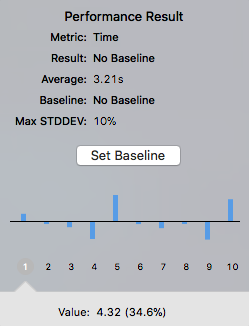
\includegraphics[width=.65\linewidth]{inc/img/perf/rsakeygen.png}
  \captionof{figure}{Результаты замеров генерации RSA ключа}
  \label{sec:eng:performance:rsakeygen:result}
\end{minipage}%
\begin{minipage}{.5\textwidth}
  \centering
  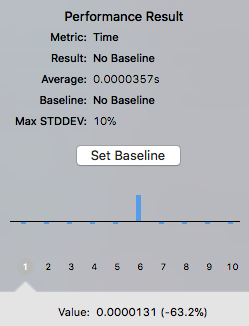
\includegraphics[width=.65\linewidth]{inc/img/perf/aeskeygen.png}
  \captionof{figure}{Результаты замеров генерации AES ключа}
  \label{sec:eng:performance:aeskeygen:result}
\end{minipage}
\end{figure}

\FPeval{\rsaKeyGenMesaureMax}{62.4}
\FPeval{\rsaKeyGenMesaureMin}{11.3}
\FPeval{\rsaKeyGenMesaureAverage}{32.1}
\FPeval{\perfDevRSAKeyGen}{clip(round((\rsaKeyGenerationMaxValue - (\rsaKeyGenMesaureMax + \rsaKeyGenMesaureMin + \rsaKeyGenMesaureMin) \ 3), 2))}

Рассчитаем отклонение от предельно допустимого значения генерации \textit{RSA} ключа, подставив значения в формулу (\ref{perfDifEquation}):
\begin{center}
\(\perfDev = \num{\rsaKeyGenerationMaxValue} - \frac{\num{\rsaKeyGenMesaureMax} + \num{\rsaKeyGenMesaureMin} + \num{\rsaKeyGenMesaureAverage}}{3} = \num{perfDevRSAKeyGen} \, \text{сек}\)
\end{center}
\subsubsection{} \textit{RSA} шифровка и расшифровка.
\label{sec:eng:performance:rsaenc}

Метод \texttt{rsaEncrypt} необходим для зашифровки данных при помощи алгоритма \textit{RSA}, а метод \texttt{rsaDecrypt} -- для расшифровки данных, зашифрованных при помощи \textit{RSA}. На рисунках \ref{sec:eng:performance:rsaenc:enc} и \ref{sec:eng:performance:rsaenc:dec} результаты измерений генерации \textit{RSA} и \textit{AES} ключей соответственно.

\begin{figure}[h]
\centering
\begin{minipage}{.5\textwidth}
  \centering
  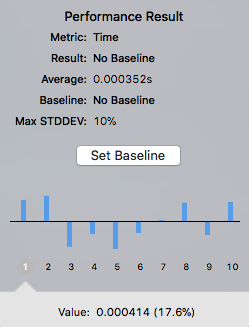
\includegraphics[width=.65\linewidth]{inc/img/perf/testRSAEncryptPerformance.png}
  \captionof{figure}{Результаты замеров шифровки при помощи RSA}
  \label{sec:eng:performance:rsaenc:enc}
\end{minipage}%
\begin{minipage}{.5\textwidth}
  \centering
  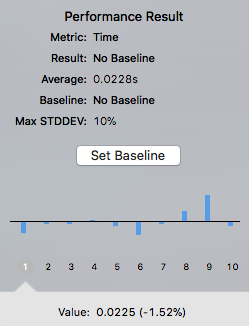
\includegraphics[width=.65\linewidth]{inc/img/perf/testRSADecryptPerformance.png}
  \captionof{figure}{Результаты замеров дешифровки при помощи RSA}
  \label{sec:eng:performance:rsaenc:dec}
\end{minipage}
\end{figure}
\subsubsection{} \textit{AES} шифровка и расшифровка.
\label{sec:eng:performance:aesenc}

Завершающей парой тестовых методов являются методы для шифровки и расшифровки при помощи алгоритма \textit{AES}: \texttt{aesEncrypt} и \texttt{aesDecrypt}. На рисунках \ref{sec:eng:performance:aesenc:enc} и \ref{sec:eng:performance:aesenc:dec} результаты измерений генерации \textit{RSA} и \textit{AES} ключей соответственно.

\begin{figure}[h]
\centering
\begin{minipage}{.5\textwidth}
  \centering
  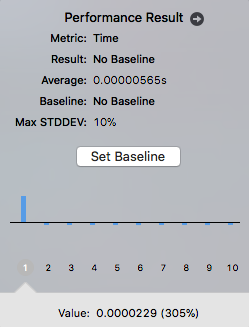
\includegraphics[width=.65\linewidth]{inc/img/perf/testAESEncryptPerformance.png}
  \captionof{figure}{Результаты замеров шифровки при помощи AES}
  \label{sec:eng:performance:aesenc:enc}
\end{minipage}%
\begin{minipage}{.5\textwidth}
  \centering
  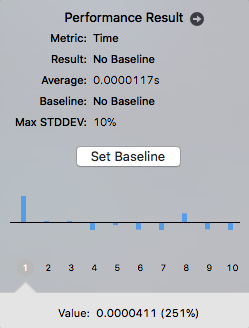
\includegraphics[width=.65\linewidth]{inc/img/perf/testAESDecryptPerformance.png}
  \captionof{figure}{Результаты замеров дешифровки при помощи AES}
  \label{sec:eng:performance:aesenc:dec}
\end{minipage}
\end{figure}


\FPeval{\aesEncMesaureMax}{0.000229}
\FPeval{\aesEncMesaureMin}{0.0000448}
\FPeval{\aesEncMesaureAverage}{0.0000565}
\FPeval{\perfAESEnc}{clip(round(((\aesEncryptMaxValue - (\aesEncMesaureMax + \aesEncMesaureMin + \aesEncMesaureAverage) / 3) / \aesEncryptMaxValue) * 100, 2))}

Рассчитаем отклонение от предельно допустимого значения времени, затраченного на шифрование при помощи \textit{AES}, подставив значения в формулу (\ref{perfDifEquation}):
\begin{center}
\(\perfDev = (\num{\aesEncryptMaxValue} - \frac{\num{\aesEncMesaureMax} + \num{\aesEncMesaureMin} + \num{\aesEncMesaureAverage}}{\num{3}}) \cdot \frac{\num{1}}{\num{\aesEncryptMaxValue}} \cdot 100 = \num{\perfAESEnc} \, \text{\%}\)
\end{center}

\FPeval{\aesDecMesaureMax}{0.000411}
\FPeval{\aesDecMesaureMin}{0.000034}
\FPeval{\aesDecMesaureAverage}{0.000117}
\FPeval{\perfAESDec}{clip(round(((\aesDecryptMaxValue - (\aesDecMesaureMax + \aesDecMesaureMin + \aesDecMesaureAverage) / 3) / \aesDecryptMaxValue) * 100, 2))}

Для дешифровки, при помощи алгоритма \textit{AES}, рассчитаем аналогичное значение:
\begin{center}
\(\perfDev = (\num{\aesDecryptMaxValue} - \frac{\num{\aesDecMesaureMax} + \num{\aesDecMesaureMin} + \num{\aesDecMesaureAverage}}{\num{3}}) \cdot \frac{\num{1}}{\num{\aesDecryptMaxValue}} \cdot 100 = \num{\perfAESDec} \, \text{\%}\)
\end{center}


В таблице \ref{sec:eng:performance:aesenc:result} приведены данные по всем измерениям. Для удобства использвоания значений, все результаты были увеличины в 10 раз. Важно отметить, что некоторые методы используются чаще остальных, поэтому разница между значениями может невилироваться частотой использования, например, генерация пары \textit{RSA} ключей выполняется только при первой авторизации в клиенте, в то время как генерация \textit{AES} ключа происходит при отправке каждого сообщения. Это же касается расшифровки сообщения: \textit{RSA} дешифрование применяется только при получении сообщения на фоновом потоке, а дальнейшее отображение (которое может повторяться столько раз, сколько сообщение будет попадать на экран) использует \textit{AES} дешифрование на главном потоке.

\begin{table}[!ht]
  \caption{Результаты расчетов производительности модуля криптографии iOS-клиента}
  \label{sec:eng:performance:aesenc:result}
  \centering
  \begin{tabularx}{\linewidth}{
    |>{\hsize=1.6\hsize}X|
    >{\centering\arraybackslash\hsize=0.8\hsize}X|
    >{\centering\arraybackslash\hsize=0.8\hsize}X|
    >{\centering\arraybackslash\hsize=0.8\hsize}X|
  }
	\hline
 \begin{center}Название метода\end{center} & Максимальное значение &  Минимальное значение &  Среднее значение \\
 \hline
 rsaKeyGeneration & \num{62.4} & \num{11.3} & \num{32.1} \\
 \hline
 aesKeyGeneration & \num{0.00323} & \num{0.0000127} & \num{0.000357} \\
 \hline
 aesEncrypt & \num{0.000229} & \num{0.0000448} & \num{0.0000565} \\
 \hline
 aesDecrypt & \num{0.000411} & \num{0.000034} & \num{0.000117} \\
 \hline
 rsaEncrypt & \num{0.00423} & \num{0.00281} & \num{0.00352} \\
 \hline
 rsaDecrypt & \num{0.236} & \num{0.224} & \num{0.228} \\
 \hline
  \end{tabularx}
\end{table}

Как видно по результатам тестов, методы, связанные с \textit{RSA} шифрованием, работают значительно медленнее аналогичных, использующих \textit{AES}. Данное поведение является ожидаемым, именно поэтому при шифровании сообщения, генерируется \textit{AES} ключ, который шифруется для каждого получателя, а само сообщение шифруется \textit{AES} ключом.